\documentclass[10pt]{beamer}

\usetheme[progressbar=frametitle]{metropolis}
\usepackage{appendixnumberbeamer}

\usepackage{booktabs}
\usepackage[scale=2]{ccicons}

\usepackage{pgfplots}
\usepgfplotslibrary{dateplot}
\usefonttheme[onlymath]{serif}
\usepackage{mathtools}
\usepackage{tikz}
\usetikzlibrary{arrows.meta, calc, fit, tikzmark}

%\usepackage{pxfonts}
%\usepackage{eulervm}


\usepackage{xspace}
\newcommand{\themename}{\textbf{\textsc{metropolis}}\xspace}

\title{First order perturbative treatment of the cosmic density-fluctuation power spectrum in the Zel’dovich approximation}
\date{07.01.2019}
\author{Thimo Preis}
% \titlegraphic{\hfill
\includegraphics[height=1.5cm]{logo.pdf}}

\begin{document}
	
	\maketitle
	
	\begin{frame}{Table of contents}
	\setbeamertemplate{section in toc}[sections numbered]
	\tableofcontents[hideallsubsections]
\end{frame}
\section{Central question}

\begin{frame}{Central question}
\begin{block}{Linear evolution of the density power spectrum}
	\begin{align}
	G^{\;\textrm{Linear}}_{\rho \rho,\;\mathrm{SPT}}(k, \tau) &= \; G^{(0), \textrm{Linear}}_{\rho \rho}\\[7pt]
	&\propto \;D^2_+ (\tau) P^{(\mathrm{i})}_{\delta}(k)\nonumber.
	\end{align} 
\end{block}
      \begin{block}{Full density power spectrum to first order in the perturbations}

	\begin{align}\label{eq:Goal}
	G^{(1)}_{\rho_1 \rho_2}& = G^{(0)}_{\rho_1 \rho_2} + \delta G_{\rho_1 \rho_2}.
	\end{align}
\end{block}

\end{frame}
\section{Kinetic Field Theory}
\begin{frame}[fragile]{Kinetic Field Theory in a nutshell}
\begin{figure}[h]
	\centering
	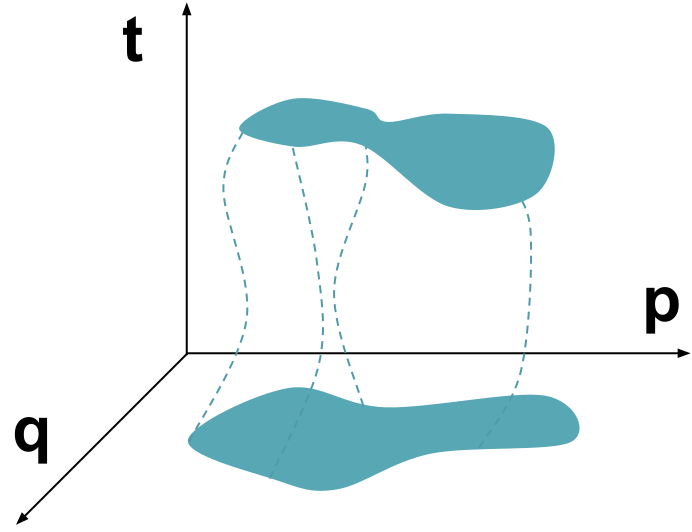
\includegraphics[width=0.6 \textwidth]{KFT.png}
	\caption{The phase-space evolution of a statistical system made up of N particles.}
\end{figure}
\begin{block}{Encoded in the canonical generating functional}
\begin{equation*}
Z_C = \int \textrm{d}\boldsymbol{ x}^{(\mathrm{i})} \, \mathcal{P}(\boldsymbol{ x}^{(\mathrm{i})})  \int_{\boldsymbol{ x}^{(\mathrm{i})}}  \mathcal{D}\boldsymbol{x} (t)  \; \delta_D\left[\boldsymbol{ x} -\boldsymbol{ x}_{\mathrm{cl}}(\boldsymbol{x}^{(\mathrm{i})})\right].
\end{equation*}

\end{block}

\end{frame}
\begin{frame}[fragile]{The Zel'dovich approximation}
\begin{block}{Equations of motion}
\begin{align}
\vec{q} \, '&=\; \vec{p}_{\mathrm{zel}} \nonumber\\
\vec{p}\,' _{\mathrm{zel}} & = \;-\; \frac{1}{g(a)}\; \vec{\nabla}_q V \; \underbrace{- \;\frac{g\,'(a)}{g(a)} \;\,\vec{p}_{\mathrm{zel}}}_{ \mathrm{drag \; force}}\label{eq:eom},
\end{align}
\end{block}
\begin{block}{Account for drag force in particle interactions}
	%\begin{equation}
	%S [\boldsymbol{\chi},\boldsymbol{ x}] = \sum_{j=1}^{N} \int_0^{\tau_f} \textrm{d}\tau_1 \; 
	%\left[\underbrace{\vec{\chi}^T_{q_j} (\vec{q}'_j-\vec{p}_{\mathrm{zel},j})+\tilde{\vec{\chi}}^T_{p_j} \vec{p}'_{\mathrm{zel},j}}_{\mathcal{L}_{0,j}}+ %\underbrace{\tilde{\vec{\chi}}^T_{p_j} \left( \frac{g'}{g} \vec{p}_{\mathrm{zel},j} + \frac{1}{g} \vec{\nabla}_{q_j} V\right)}_{\mathcal{L}_{\mathrm{I},j}}\right],
	%\end{equation}
	\vspace{0.3 cm}
	\begin{equation}
	S_{\mathrm{I}} = \;S_{\mathrm{V}} \;+\; S_{\mathrm{D}},
	\end{equation}
\end{block}
\end{frame}
\begin{frame}[fragile]{The Zel'dovich approximation within Kinetic Field Theory}

\begin{block}{The canonical generating functional}
	\vspace{0.2cm}
\begin{equation}
	Z_C \left[\boldsymbol{J}, \boldsymbol{K}, \mathrm{H}\right]=\; e^{i \hat{S}_I}\; e^{i \,\mathrm{H} \cdot \hat{ \Phi}}\; Z_{C, 0} [\boldsymbol{J}, \boldsymbol{K}].	
\end{equation}

\end{block}
\vspace{1.4 cm}
\begin{block}{Perturbative corrections to the density power spectrum}
	\vspace{0.2 cm}
	\begin{equation}
		\delta G_{\rho_1 \rho_2} = \; \delta G^{ \mathrm{V}}_{\rho_1 \rho_2} \; + \; \delta G^{\mathrm{D}}_{\rho_1 \rho_2}.
	\end{equation}
\end{block}
\end{frame}
\section{The density power spectrum to first order in the perturbations}



  \begin{frame}[fragile]{The drag cumulant}

  		\begin{columns}
	\column{0.3 \linewidth}
	\begin{align*}
\delta G^{ \mathrm{D}}_{\rho_1 \rho_2}&=\; \alert{\delta G^{ \mathrm{D},1}_{\rho_1 \rho_2}} \; \\[7pt]
&+\; \delta G^{ \mathrm{D},2}_{\rho_1 \rho_2}.
	\end{align*}
	\column{0.7 \linewidth}
	\begin{figure}
	\includegraphics[width=0.92 \textwidth]{../figures/ComparisonDragcum2ContributionsFreePS.pdf}
\caption{Comparison of the first contribution to the drag cumulant with the free density cumulant.}
		
	\end{figure}
	
\end{columns}

\end{frame}
  \begin{frame}[fragile]{The drag cumulant}

\begin{columns}
	\column{0.3 \linewidth}
	\begin{align*}
	\delta G^{ \mathrm{D}}_{\rho_1 \rho_2}&=\; \delta G^{ \mathrm{D},1}_{\rho_1 \rho_2}\; \\[7pt]
	&+\; \alert{\delta G^{ \mathrm{D},2}_{\rho_1 \rho_2}}.
	\end{align*}
	\column{0.7 \linewidth}
	\begin{figure}
		\includegraphics[width=0.92 \textwidth]{../figures/ComparisonDragcum3ContributionsFreePS.pdf}
		\caption{Comparison of the second contribution to the drag cumulant with the free density cumulant.}
		
	\end{figure}
	
\end{columns}

\end{frame}

\begin{frame}[fragile]{Comparison of drag and interaction cumulant}
\begin{columns}
	\column{0.3 \linewidth}
	\begin{equation*}
	- \;\delta G^{ \mathrm{D},\mathrm{Linear}}_{\rho_1 \rho_2} \;\approx \;\delta G^{ \mathrm{V}, \mathrm{Linear}}_{\rho_1 \rho_2}.
	\end{equation*}
	\column{0.7 \linewidth}
	\begin{figure}
		\includegraphics[width=0.9 \textwidth]{../figures/ComparisonInteractingDragCumulant.pdf}
		\caption{Comparison of the interaction and the full drag cumulant.}
		
	\end{figure}
	
\end{columns}

\end{frame}

\begin{frame}[fragile]{The full first order perturbed density power spectrum}
	\begin{figure}[h]
		\centering
		\includegraphics[width=0.7\paperheight]{../figures/FullPerturbedPS.pdf}
		\caption{Free and first order perturbative contributions to the density-fluctuation power spectrum.}
		\label{fig:comparison_fullPS}
	\end{figure}
\end{frame}
\section{Conclusion}
\begin{frame}[fragile]{Conclusion}
	\begin{enumerate}
		\item KFT employing a Zel'dovich approximation reproduces the growth behaviour obtained from conventional approaches in the \textbf{linear} regime.
		\vspace{0.5 cm}
		\item Qualitatively, the behaviour in the \textbf{non-linear} regime of the $\Lambda$CDM density power spectrum is recreated.
		\vspace{0.5 cm}
		\item It remains to be seen whether this result holds true in next-to-leading order perturbation theory.
	\end{enumerate}
\end{frame}
\appendix

\begin{frame}{Final density power spectrum}
	\begin{figure}
		\centering
		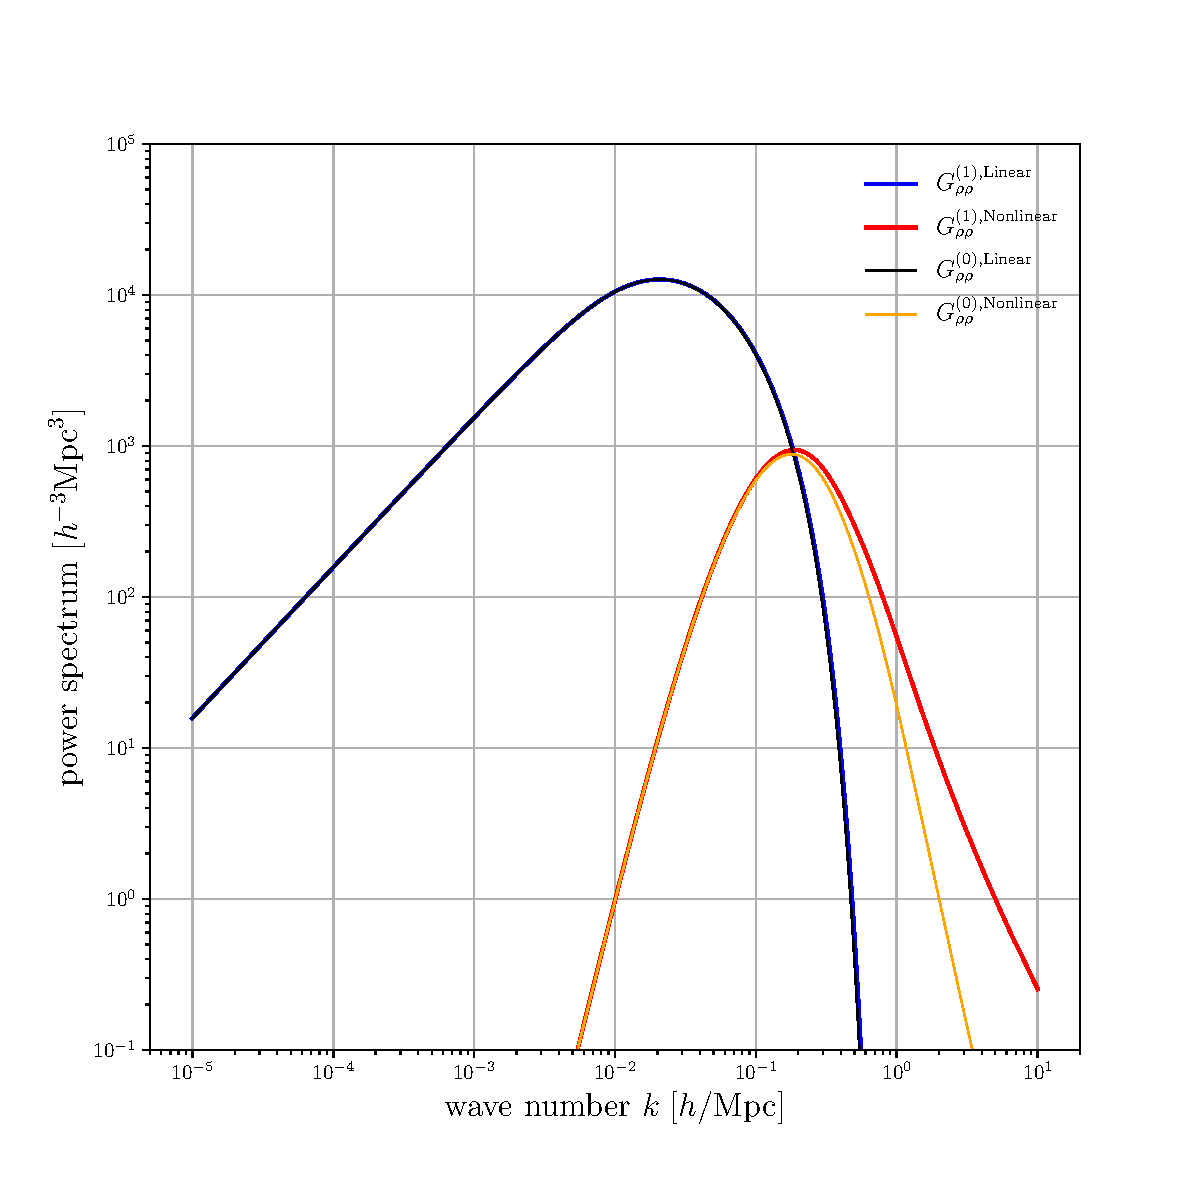
\includegraphics[width=0.65\textwidth]{FullPerturbedPSLinearAndNonlinear.pdf}
		\caption{Linear and non-linear contributions to the density power spectrum to zeroth and first order in the perturbations.}
	\end{figure}
\end{frame}

\begin{frame}{The drag field}
	\begin{block}{Drag field in Fourier space}
		\begin{align*}
		S_D &= \int \textrm{d}1 \; \sum_{j=1}^{N} \vec{\chi}_{p_j}(\tau_1) \delta_D(\vec{x}_1 - \vec{x}_j (\tau_1)) \underbrace{\frac{g'}{g}(\tau_1)}_{:= A_D (\tau_1)} \vec{p}_1 =: \int \textrm{d}1 \; \Phi_D (1)\\
		\hat{\Phi}_D (1)& = \sum_{j=1}^{N}  A_D (\tau_1) (2\pi)^6 \delta_D(\vec{k}_1) \left(\frac{\partial}{i \partial \vec{l}_1} \delta_D(\vec{l}_1)\right) \hat{\vec{\chi}}_{p_j} (\tau_1)\hat{ \Phi}_{f_j}(1) \\
		&=: \sum_{j=1}^{N} \hat{ d} _j (1) \hat{ \Phi}_{f_j}(1), 
		\end{align*}
	\end{block}
\end{frame}
\begin{frame}{The interaction or non-mode-coupling cumulant}
%	\begin{block}{Symmetric contribution of the non-mode-coupling cumulants}
		\begin{columns}
		\column{0.3 \linewidth}
		\textbf{Symmetric contribution of the non-mode-coupling cumulants}
			\begin{equation*}
					    	4 i \int \textrm{d}\bar{2} \; G^{(0,1)}_{\rho_{\bar{1}} \mathcal{F}_{\bar{2}}} G^{(0,2)}_{\rho_{\bar{2}} \rho_2}  
			\end{equation*}
		\column{0.7 \linewidth}
					\begin{figure}
					\includegraphics[width=0.9\textwidth]{../figures/CompIntDragfreePSInt.pdf}
						\caption{ Linear and non-linear contributions in the initial power spectrum to the interacting cumulant.}
					
				     \end{figure}

			\end{columns}
\end{frame}
\begin{frame}{The initial power spectrum}
\begin{block}{Bardeen, Bond, Kaiser and
		Szalay (BBKS) }
	\begin{equation*}
	P^{(\mathrm{i})}_{\delta}(k):= P_{\delta}(\vec{k}, t_i)  \propto
	\begin{cases}
	k^{n_s} & (k  \ll k_{eq})\\
	k^{n_s -4} & (k \gg k_{eq})
	\end{cases}
	\qquad
	\Rightarrow
	P^{(\mathrm{i})}_{\delta}(k) \propto k^{n_s}\, T^2(k),
	\end{equation*}
	\begin{figure}
		\centering
		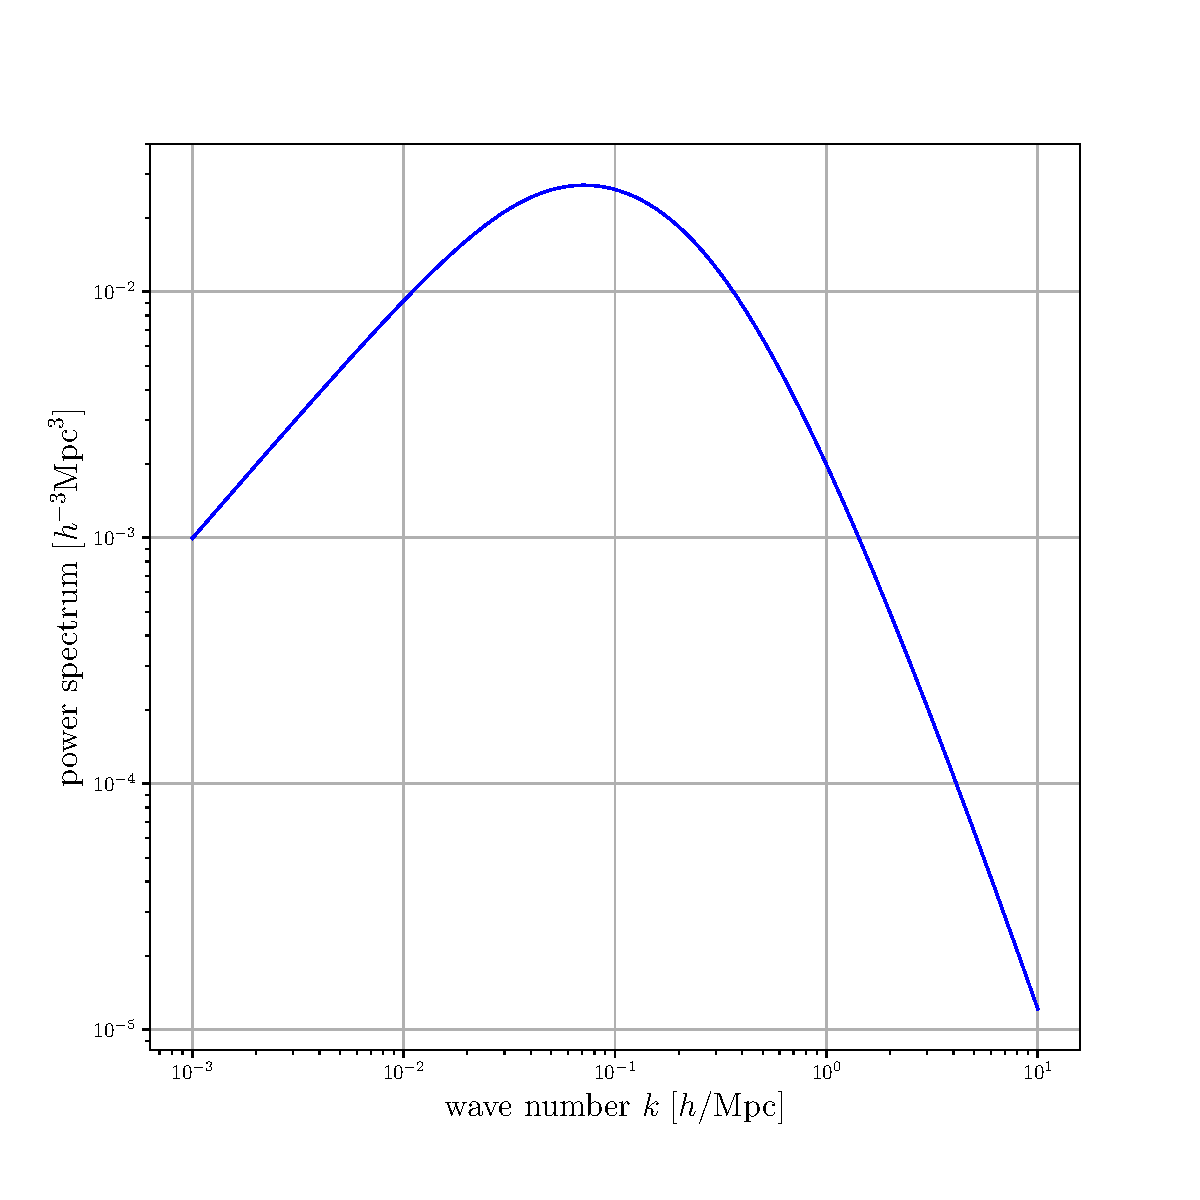
\includegraphics[width=0.365 \textwidth]{Bardeenps.pdf}
		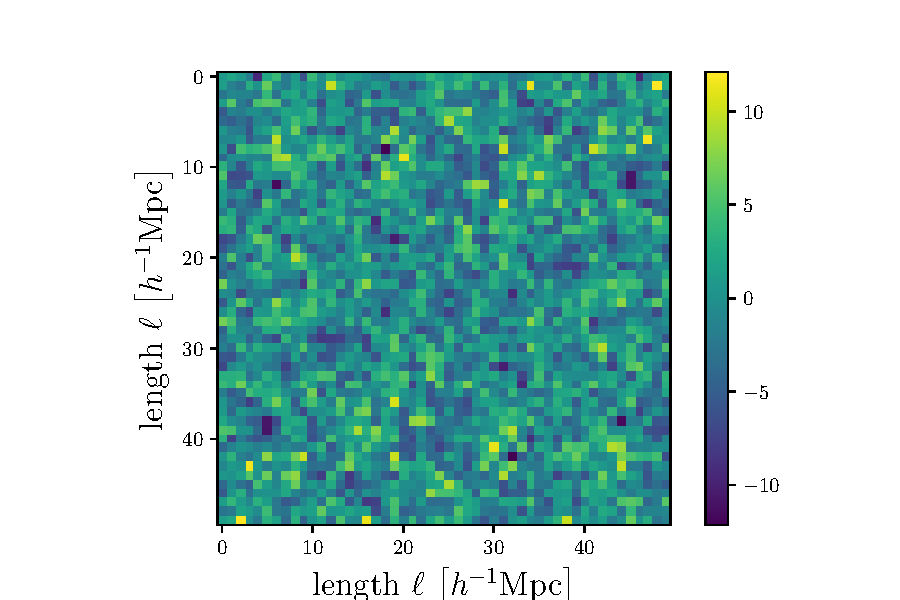
\includegraphics[width=0.55 \textwidth]{InitialConfigurationRealSpace.pdf}
		\caption{Left: Initial power spectrum by Bardeen et al., Right: Initial configuration in real space for EdS.}
	\end{figure}
	
\end{block}
\end{frame}
{%
\setbeamertemplate{frame footer}{Source: Baumann Cambridge Lecture \textbf{Cosmology} Mathematical Tripos III}
\begin{frame}{Perturbations in the radiation-dominated era}
	\begin{figure}
		\centering
		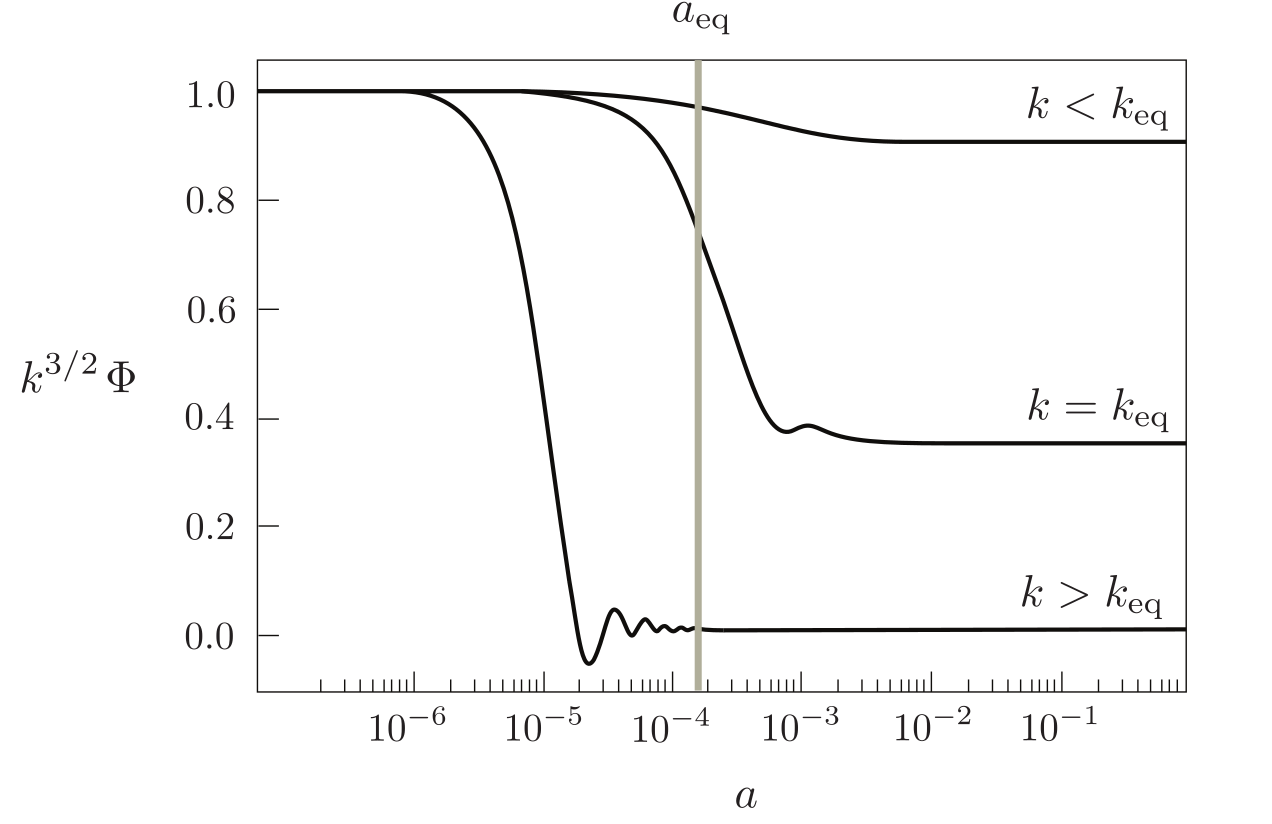
\includegraphics[width=0.9 \textwidth]{PerturbationsRadiationEra.png}
		\caption{Numerical solutions for the linear evolution of the gravitational potential.}
	\end{figure}

\end{frame}
}
{%
\setbeamertemplate{frame footer}{Source: Baumann Cambridge Lecture \textbf{Cosmology} Mathematical Tripos III}
\begin{frame}{Measurements}
\begin{figure}
	\centering
	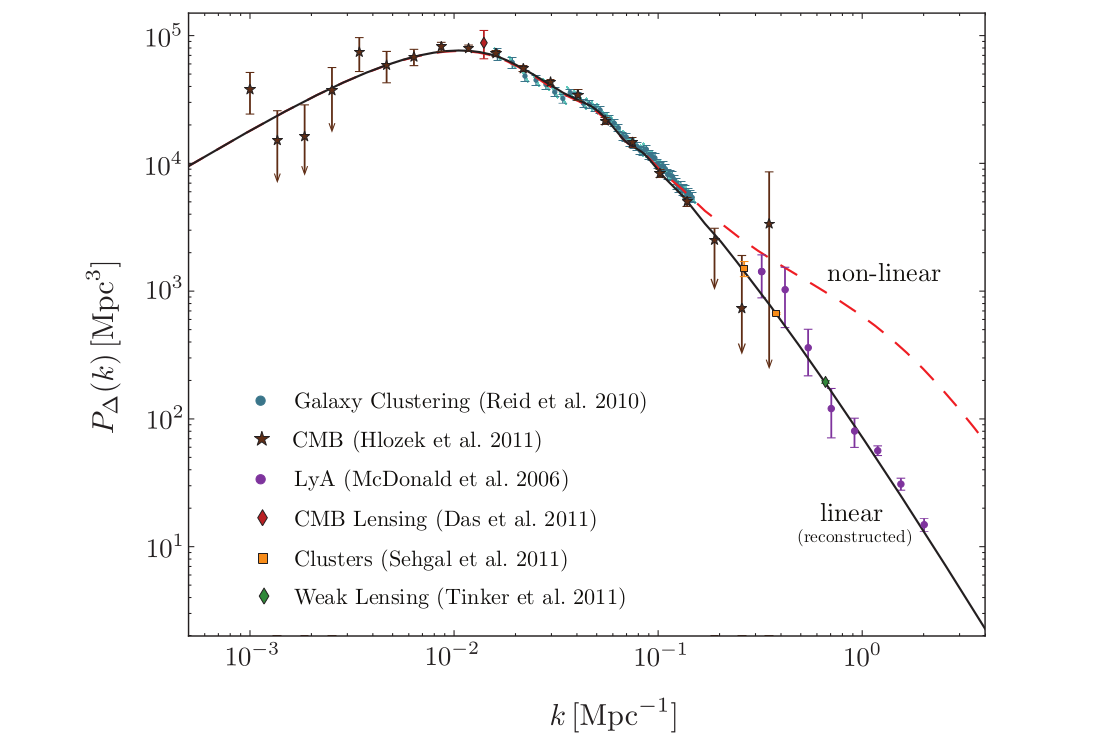
\includegraphics[width=0.9 \textwidth]{MatterPowerSpectrumToday.png}
	\caption{Collection of measurements of the $\Lambda$CDM matter power spectrum.}
	
\end{figure}
\end{frame}
}
\begin{frame}{On the calculation of cumulants}
	\begin{align}
		G_{ab} &= \hat{ H}_a \hat{ H}_b \ln{Z_C [H, J, K]}_0 = \hat{ H}_a \left(\frac{1}{Z_C} e^{i \hat{S}_I} W^{(0)}_b e^{W^{(0)}}\right)_0\\
		&= \frac{1}{Z_C[0]} e^{i \hat{S}_I}\left(W^{(0)}_{ab} + W^{(0)}_a W^{(0)}_b\right)e^{W^{(0)}} \mid_0 \nonumber \\
		&-\frac{1}{Z^2_C[0]} \left(e^{i \hat{S}_I} W^{(0)}_a e^{W^{(0)}} \right) \left(e^{\hat{S}_I} W^{(0)}_b  e^{W^{(0)}}\right)_0
	\end{align}
	Then use the following relation after applying all neccessary derivatives to identify cumulants:
	\begin{equation}
	W^{(0)}_{a_1 \dots a_n} \mid_0 = G^{(0)}_{a_1 \dots a_n}
	\end{equation}
\end{frame}
\end{document}
